\chapter{Introduction}
Natural products (NPs) are organic compounds derived from biological sources, showcasing
diverse bioactivities and serving as crucial reservoirs for novel drug discovery. Their chemical
structures range from simple to complex molecules \cite{Thirumurugan2018}. Primary metabolites are vital for an
organism’s growth, development, and reproduction, while secondary metabolites, arising from
cell communication and environmental adaptation, are not essential for these processes but are
integral for defense mechanisms \cite{MShuikan2021}. Countless secondary metabolites find applications in
medicine, agriculture, and manufacturing, with over 2,140,000 known compounds catego-
rized by biosynthesis mode into six main classes: terpenoids, fatty acid-derived substances,
polyketides, alkaloids, nonribosomal and ribosomal polypeptides, and enzyme cofactors \cite{Nicolaou2017}.\\


Fungi, plants, and bacteria are key kingdoms with well-developed secondary metabolism, contributing to the production of around 500,000 known secondary metabolites. 
Among these, microbes produced for 70,000, with fungi producing nearly 47\% of microbial bioactive compounds \cite{Bills2016}. The rate of discovery of fungal metabolites has increased significantly, especially in filamentous fungi like Ascomycota and Basidiomycota. These metabolites, crucial for fungi's ecological success, exhibit diverse biological activities, ranging from harmful mycotoxins to beneficial pharmaceuticals. Fungal secondary metabolites have been utilized to create therapeutic agents and lead compounds for treating various conditions, including cancer, bacterial and fungal infections, autoimmune diseases, and neurological and cardiovascular disorders. Notable examples include $\beta$-lactam antibiotics like penicillins and cephalosporins. Beyond their medical applications, these metabolites have also played a role in the development of new pesticides and biomolecular probes \cite{Bills2016}. While fungal metabolites have revolutionized medicine and agriculture, much of fungal biodiversity remains unexplored, suggesting vast potential for discovering new bioactive compounds \cite{Bills2016}.\\


The fundamental steps in the discovery of natural products, such as organism isolation, identification, preservation, fermentation screening, and extract preparation, have remained consistent over time. Bioassay-guided separation and structure elucidation of active compounds became standard in the 1950s \cite{Karwehl2016}. In recent research on secondary metabolites, new techniques like genome mining and biodiversity exploration have been added to the process. The workflow still begins with collecting fungi, but accurate taxonomic classification is crucial, as it can influence secondary metabolite production. Understanding fungal ecology is also important, as it affects metabolite synthesis, such as in cases of horizontal gene transfer from bacteria to fungi. Genome sequencing can identify gene loci responsible for secondary metabolite biosynthesis. Modulating biosynthesis through DNA methylation or enzyme knockouts is another strategy. Additionally, cultivation media play a vital role in compound production, with the use of different media potentially leading to new secondary metabolites. Optimizing conditions for scaling up fermentation is also critical \cite{Karwehl2016}.


\begin{figure}[H]
    \centering
    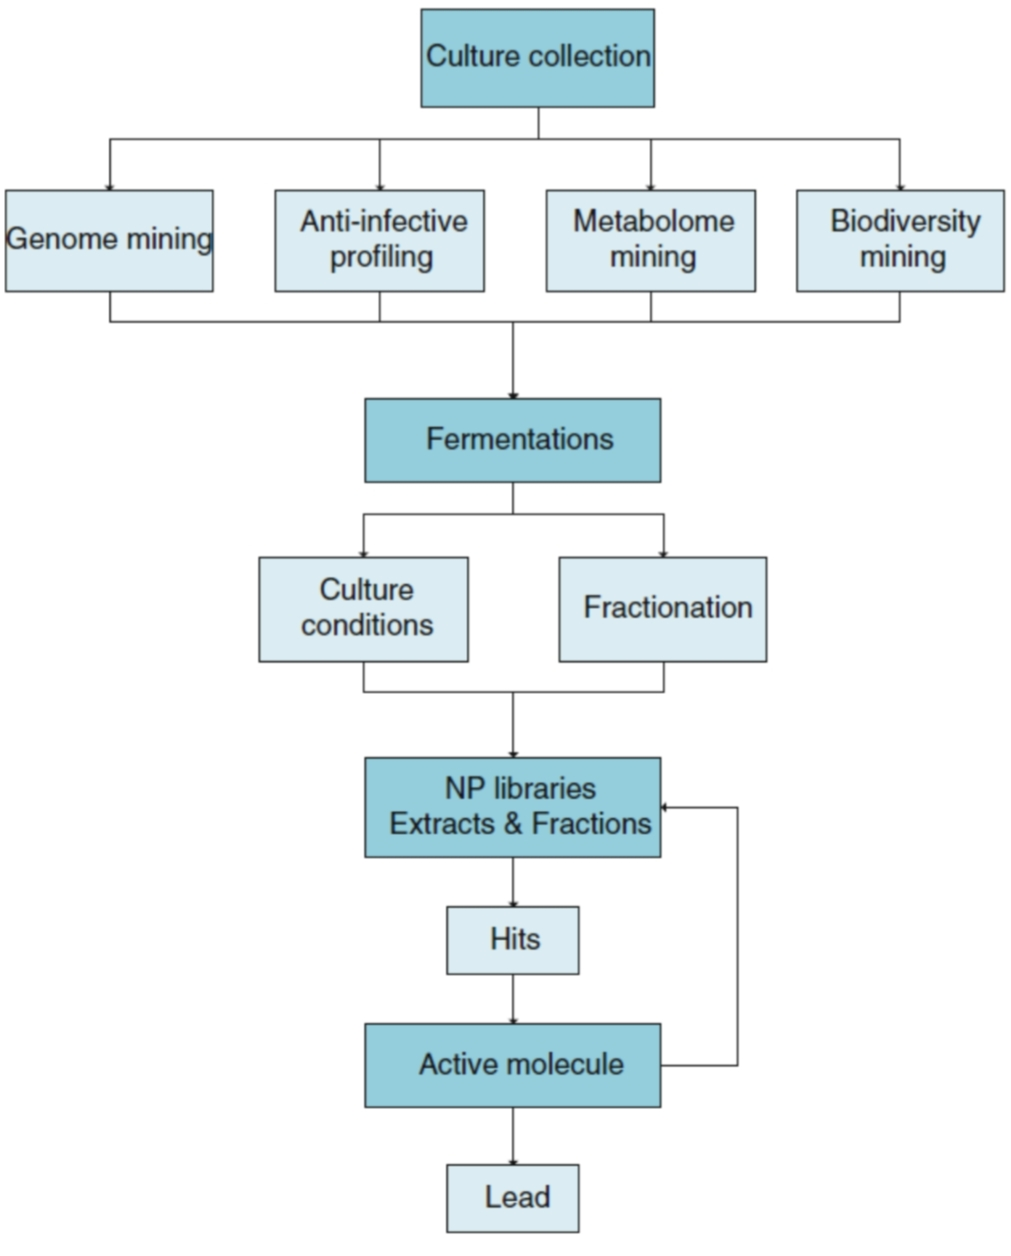
\includegraphics[width=8cm]{images/introduction/intro-flow-chart.jpg}
    \caption{General workflow for antibiotic natural product discovery \cite{Karwehl2016}}
    \label{}
\end{figure}


Basidiomycota, the second-largest fungal phylum with around 40,000 species, has been a significant source of bioactive metabolites. Molecular phylogenetic studies have expanded species recognition, with an estimated 54,000 species by 2030. Most research has focused on Agaricomycetes, while other classes like Ustilagomycetes remain understudied \cite{He2019-time}. Basidiomycota are also the source of various unique secondary metabolites, of which a handful have made it into development as agrochemical pesticides or pharmaceutical lead structures, as exemplified by the cytotoxic illudins, the antifungal strobilurins and the antibacterial pleuromutilins \cite{He2019-time}. Basidiomycota, particularly mushrooms, have long been used in traditional medicine and food. Their economic value in various bio-economies is significant, with fungi contributing an estimated USD 54.57 trillion annually \cite{Sum2023-vinni}. Advances in biotechnology and analytics have led to the discovery of novel bioactive compounds such as monoterpenoids and polyynes,sesquiterpenoids, diterpenoids,triterpenoids, tetraterpenoids, polyketides and mixed terpenes ,alkaloids and peptides and research continues to explore Basidiomycota's chemical diversity and pharmaceutical potential (anti-inflammatory effects, antitumor effects, antifungal activities, immunosuppressive effects, anticancer activities). Artemisinin, Thapsigargin, and Paclitaxel are clinically approved compounds utilized for medical purposes \cite{Bergman2019}.\\

Cyclocybe aegerita is a significant fungal species also known as the poplar mushroom or black mushroom due to its practical applications. First, it is an edible mushroom widely  grown on dead hardwood particularly poplar, willow, other related trees and  cultivated on an industrial scale, prized for its exceptional aroma and meaty texture \cite{Surup2019}. Additionally, it has long served as a model organism in microbiological and genetic research, particularly in studies on fruiting body development \cite{Surup2019}.\\


Cyclocybe aegerita is commonly cultivated for culinary purposes, particularly in Asian and Mediterranean cuisine \cite{wikipedia}. The mushroom has a smooth, brownish cap, and its gills change color as the mushroom matures, producing a white spore print. This species is native to regions of Europe, Asia, and parts of North America \cite{wikipedia}.\\

In this study, monokaryotic and dikaryotic strains of C. aegerita were examined, including strains AAE-3, AAE-3-32, AAE-3-40, AAE-3-37, and AAE-3-24. The dikaryotic strain AAE-3 successfully produced fruiting bodies and basidiospores under controlled conditions. However, none of the monokaryotic strains exhibited sexual sporulation, as indicated by the absence of spore prints surrounding the fruiting bodies \cite{Orban2020}. Strain AAE-3-32 was identified as an abortive + true homokaryotic fruiting type (AHF+THF). AAE-3-40 and AAE-3-37 were classified as "initials type" and "elongated initials type," respectively, while AAE-3-24 was characterized as a mycelium type \cite{Herzog2016}.\\

Terpenes and terpenoids are a large and diverse class of natural products, with over 80,000 known compounds. These secondary metabolites have various structures and functions. They are divided into classes based on the number of isoprene units into groups like hemi-, mono-, sesqui-, di-, sester-, and triterpenes. Terpenoids are altered forms of terpenes, frequently by adding oxygen, whereas "terpenes" are the direct results of terpene synthases.\\

All terpenes originate from two pathways: the methyl erythritol 4-phosphate (MEP) pathway and the mevalonate (MVA) pathway. Both lead to the formation of two key compounds, dimethylallyl diphosphate (DMAPP) and isopentenyl diphosphate (IPP). These are further processed by prenyltransferases into intermediates such as geranyl diphosphate (GPP), farnesyl diphosphate (FPP), and geranylgeranyl diphosphate (GGPP), which serve as substrates for terpene synthases. The diversity of terpene structures produced by these enzymes can be further enhanced by post-modification processes like oxidation.\\

Terpenes and terpenoids are of special interest due to their wide range of  potential applications. Traditionally, they have been used in essential oils and plant extracts for medicinal purposes. Even today, terpenes play key roles in medicine. For instance, paclitaxel, a diterpenoid from yew trees (Taxus spp.), is essential in the treatment of cancer, whereas artemisinin, a sesquiterpenoid from Artemisia annua, is a key drug for malaria. In addition to their medicinal  applications, terpenes contribute to flavors and fragrances in foods and perfumes, such as the grapefruit-like nootkatone and the citrus-scented limonene.\\

While most terpenes have been discovered in plants, they are present in all organisms, including fungi. Fungi, due to their vast species diversity and adaptability, are highly promising for producing novel terpenes and terpenoids. Their ability to produce a wide range of bioactive secondary metabolites present prospects for isolation of new compounds with various applications, covering from medicine to biofuels.
